\documentclass[11pt,tikz,border=3mm]{standalone}
\usepackage{amsmath}
\usetikzlibrary{arrows.meta}
\definecolor{ink}{HTML}{263244}
\definecolor{bluefill}{HTML}{DBEAFE}
\definecolor{blueedge}{HTML}{2563EB}
\definecolor{amberfill}{HTML}{FEF3C7}
\definecolor{amberedge}{HTML}{D97706}
\definecolor{redfill}{HTML}{FEE2E2}
\definecolor{rededge}{HTML}{DC2626}
\definecolor{greenfill}{HTML}{E5F3E9}
\definecolor{greenedge}{HTML}{368053}
\tikzset{
  font=\sffamily\normalsize,
  >={Latex[length=2mm]},
  block/.style={draw=ink,rounded corners=2pt,align=center,minimum height=10mm,inner sep=2pt},
  ftm/.style={block,draw=blueedge,fill=bluefill,line width=1pt,minimum width=20mm},
  itm/.style={block,draw=amberedge,fill=amberfill,line width=1pt,minimum width=20mm},
  head/.style={block,draw=rededge,fill=redfill,line width=1pt,minimum width=25mm},
  future/.style={block,draw=greenedge,fill=greenfill,minimum width=26mm},
  flow/.style={->,draw=ink,line width=.9pt},
  control/.style={->,draw=greenedge,dashed,line width=.9pt},
  direct/.style={->,draw=blueedge,dashed,line width=.9pt}
}
\begin{document}
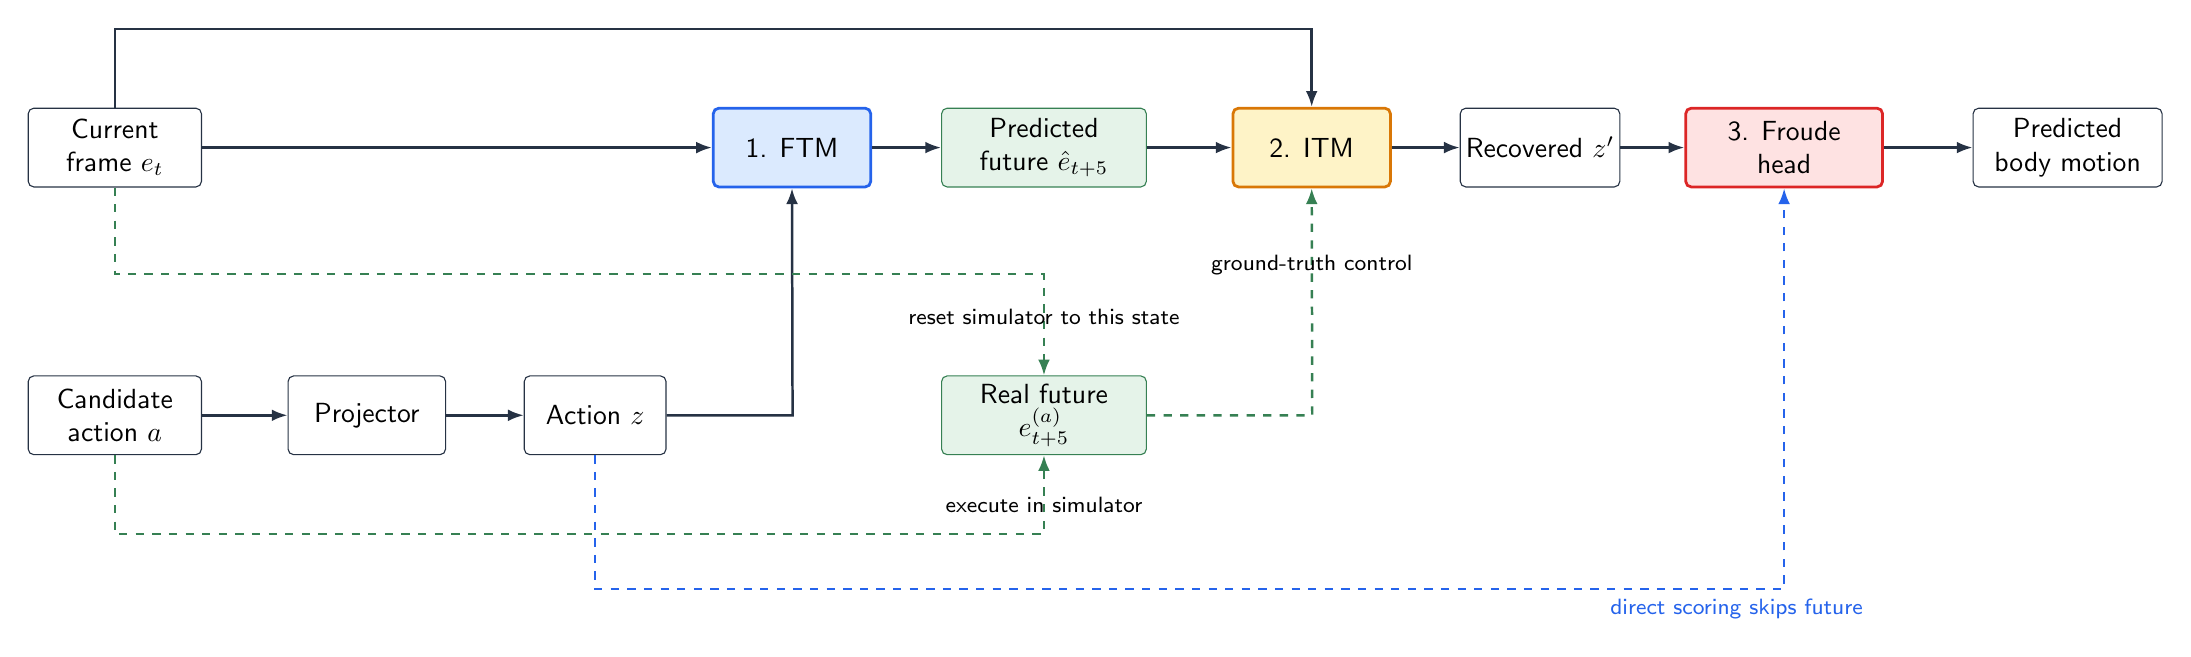
\begin{tikzpicture}[x=1mm,y=1mm]
  \node[block,minimum width=22mm] (e) at (14,62) {Current\\frame $e_t$};
  \node[block,minimum width=22mm] (a) at (14,28) {Candidate\\action $a$};
  \node[block,minimum width=20mm] (p) at (46,28) {Projector};
  \node[block,minimum width=18mm] (z) at (75,28) {Action $z$};
  \node[ftm] (f) at (100,62) {1. FTM};
  \node[future] (q) at (132,62) {Predicted\\future $\hat e_{t+5}$};
  \node[future] (s) at (132,28) {Real future\\$e^{(a)}_{t+5}$};
  \node[itm] (i) at (166,62) {2. ITM};
  \node[block,minimum width=18mm] (zp) at (195,62) {Recovered $z'$};
  \node[head] (h) at (226,62) {3. Froude\\head};
  \node[block,minimum width=24mm] (v) at (262,62) {Predicted\\body motion};

  % Exactly the Mermaid edges: both future frames enter the same ITM.
  \draw[flow] (a)--(p);
  \draw[flow] (p)--(z);
  \draw[flow] (z.east) --++(16,0) -- (f.south);
  \draw[flow] (e.east) -- (f.west);
  \draw[flow] (f)--(q);
  \draw[flow] (q)--(i);
  \draw[flow] (e.north) -- ++(0,10) -| (i.north);
  \draw[control] (a.south) -- ++(0,-10) -| node[pos=.80,below,font=\sffamily\footnotesize]{execute in simulator} (s.south);
  \draw[control] (e.south) -- ++(0,-11) -| node[pos=.80,above,font=\sffamily\footnotesize]{reset simulator to this state} (s.north);
  \draw[control] (s.east) -- ++(21,0) -- node[pos=.75,below,font=\sffamily\footnotesize]{ground-truth control} (i.south);
  \draw[flow] (i)--(zp);
  \draw[flow] (zp)--(h);
  \draw[flow] (h)--(v);
  \draw[direct] (z.south) -- ++(0,-17) -| node[pos=.48,below,font=\sffamily\footnotesize,text=blueedge]{direct scoring skips future} (h.south);
\end{tikzpicture}
\end{document}
